\section*{Exercice 189 -- Modélisation}
\setcounter{exo}{0}
%Ecole de l'air PSI 2002
On considère que l’atterrisseur est constitué de deux solides en liaison encastrement :
\begin{itemize}
\item solide 1’ : roue de centre $I$, de masse $m_{1’}$, assimilée à un fil de section négligeable formant un cercle de rayon $r_{1’}$ dans le plan $\left(I,\vect{x_1},\vect{z_1}, \right)$ avec $\vect{z}=\vect{z_1}$;
\item fourreau 1’’ : tube plein homogène cylindrique d’axe $\vect{HO}$, de rayon $r_{1''}$ et de masse $m_{1''}$;
 \end{itemize}
avec $\vect{IH}=d\vect{y_1}$ et $\vect{OH}\wedge \vect{z_1}=\vect{0}$.

\begin{center}
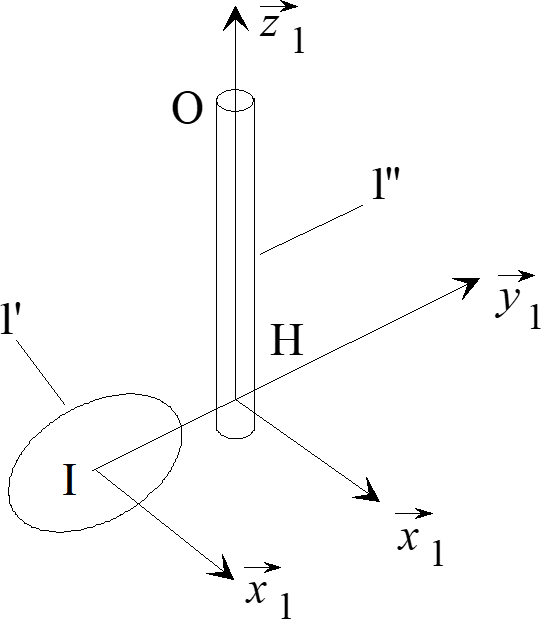
\includegraphics[width=\linewidth]{974_01}%
\end{center}


On note $\inertie{I}{1'}=\matinertie{A_{1'}}{B_{1'}}{C_{1'}}{-D_{1'}}{-E_{1'}}{-F_{1'}}{\base{x_1}{y_1}{z_1}}$ 
la représentation la plus générale de l’opérateur d’inertie de la roue 1'.


\subparagraph{}
\textit{En utilisant les propriétés géométriques de la pièce 1’, donner une écriture générale simplifiée de $\inertie{J}{1'}$.}
\ifprof
\begin{corrige}
\end{corrige}
\else
\fi

\subparagraph{}
\textit{Déterminer l’inertie du solide 1’, par rapport à l’axe $\axe{I}{z_1}$ en fonction de $m_{1'}$ et $r_{1'}$.}
\ifprof
\begin{corrige}
\end{corrige}
\else
\fi

\subparagraph{}
\textit{En déduire l’inertie du solide 1’, par rapport à l’axe $\axe{O}{z_1}$ en fonction de $d$, $m_{1'}$ et $r_{1'}$.}
\ifprof
\begin{corrige}
\end{corrige}
\else
\fi

\subparagraph{}
\textit{Déterminer l’inertie du solide 1'', par rapport à l’axe $\axe{O}{z_1}$ en fonction de $m_{1''}$ et $r_{1''}$.}
\ifprof
\begin{corrige}
\end{corrige}
\else
\fi


\subparagraph{}
\textit{En déduire l’inertie du solide $1=1'\cup 1''$, par rapport à l’axe $\axe{O}{z_1}$.}
\ifprof
\begin{corrige}
\end{corrige}
\else
\fi




\begin{enumerate}
\item $\inertie{J}{1'}=\matinertie{A_{1'}}{C_{1'}}{C_{1'}}{0}{0}{0}{}$.
\item $C_{1'}=\dfrac{m_{1'}r_{1'}^2}{2}$.
\item $C_{1'}'=C_{1'}+m_{1'}d^2=m_{1'}\left(\dfrac{r_{1'}^2}{2}+d^2\right)$.
\item $C_{1''}=\dfrac{m_{1''}r_{1''}^2}{2}$.
\item $J=\dfrac{m_{1''}r_{1''}^2}{2}+m_{1'}\left(\dfrac{r_{1'}^2}{2}+d^2\right)$.
\end{enumerate}